\section{The Identity-Transformation Approach}
\label{sec:challenge}

%We discuss the security requirements of privacy-preserving SSO and present the identity-transformation approach.

\subsection{Security Requirements for SSO Services}
\label{subsec:basicrequirements}

Non-anonymous SSO services \cite{OpenIDConnect,rfc6749,SAML,SAMLIdentifier,NIST2017draft} are designed to allow a user to log into an honest RP with her account at this RP, %correlating multiple logins,
by presenting \emph{identity tokens} issued by a trusted IdP.

To achieve this goal, the IdP issues an identity token that specifies the visited RP (i.e., \emph{RP designation}) and identifies the authenticated user (i.e., \emph{user identification})
        by (pseudo-)identities \cite{OpenIDConnect,rfc6749,SAML}.
An honest RP checks the RP's identity enclosed in a token before accepting it and allows the token holder to log in as the specified account. This prevents malicious RPs from replaying received tokens to gain illegal access to other honest RPs as victim users.

\emph{Authenticity}, \emph{confidentiality}, and \emph{integrity} of identity tokens are necessary to prevent forging, eavesdropping and tampering.
Identity tokens are signed by the trusted IdP,
    transmitted over HTTPS \cite{OpenIDConnect, rfc6749, SAML},
    and finally forwarded to target RPs by the authenticated user.
Regular security mechanisms in a browser (e.g., HTTP session and \verb+postMessage+ targetOrigin)
are also required for confidentiality of tokens \cite{GoogleIdIntegrate,de2014oauth,FettKS14,BrowserID} (see Section \ref{sec:web-design} for details).

%The requirements for secure SSO services, i.e., RP designation, user identification, integrity, and confidentiality of identity tokens, have been extensively studied \cite{ArmandoCCCT08, SPRESSO, FettKS14, FettKS16, FettKS17}.
%Any vulnerabilities that undermine these properties result in various attacks \cite{SomorovskyMSKJ12, WangCW12, ArmandoCCCPS13, ZhouE14, WangZLLYLG15, WangZLG16, YangLLZH16, MainkaMS16, MainkaMSW17, YangLCZ18, YangLS17, ShiWL19, ChenPCTKT14, ccsSunB12, DiscoveringJCS, dimvaLiM16, CaoSBKVC14, TowardsShehabM14}.

\begin{table}[t]
\footnotesize
    \caption{The (pseudo-)identities in \usso}
    \centering
%    \begin{tabular}{|l|l|l|}
    \begin{tabular}{|l|p{5.215cm}|l|} \hline
    {\textbf{Notation}} & {\textbf{Description}} & {\textbf{Lifecycle}} \\ \hline
    {$ID_{U_i}$} & {The $i$-th user's unique identity at the IdP.} & {Permanent} \\ \hline
    {$ID_{RP_j}$} & {The $j$-th RP's unique identity at the IdP.} & {Permanent} \\ \hline
    {$PID_{U_i,j}^l$} & {The $i$-th user's pseudo-identity in her $l$-th login visiting the $j$-th RP.} & {Ephemeral} \\ \hline
    {$PID_{RP_j}^l$} & {The $j$-th RP's pseudo-identity in the user's $l$-th login visiting this RP.} & {Ephemeral} \\ \hline
    {$Acct_{i,j}$} & {The $i$-th user's account at the $j$-th RP.} & {Permanent} \\ \hline
    \end{tabular}
    \label{tbl:notations-dilemma}
\end{table}


\subsection{Identity Transformation}
\label{subsec:solutions}

\usso\ implements privacy-preserving SSO that ensures security as above, while preventing both IdP-based login tracing and RP-based identity linkage.
The requirements of security and privacy are satisfied through \emph{transformed identities} in the identity tokens. Table \ref{tbl:notations-dilemma} lists the notations,
and a sub/super-script (i.e., $i$, $j$, or $l$) may be omitted if it does not cause ambiguity.


A user initiates a login by negotiating an \emph{ephemeral} pseudo-identity $PID_{RP}$  with the target RP and sending an identity-token request for $PID_{RP}$ to an IdP.
After successfully authenticating the user as $ID_U$, the IdP calculates an \emph{ephemeral} $PID_U$ based on $ID_U$ and $PID_{RP}$ and then issues an identity token that binds $PID_U$ and $PID_{RP}$.
On receiving a verified token, the RP calculates the user's \emph{permanent} $Acct$ and allows the token holder to log in.
The relationships among the (pseudo-)identities are depicted in Figure \ref{fig:IDCorrelation}.
Red and green blocks represent \emph{permanent} identities and \emph{ephemeral} pseudo-identities, respectively, and 
labeled arrows denote the transformations of (pseudo-)identities.

\begin{figure}[b]
  \centering
  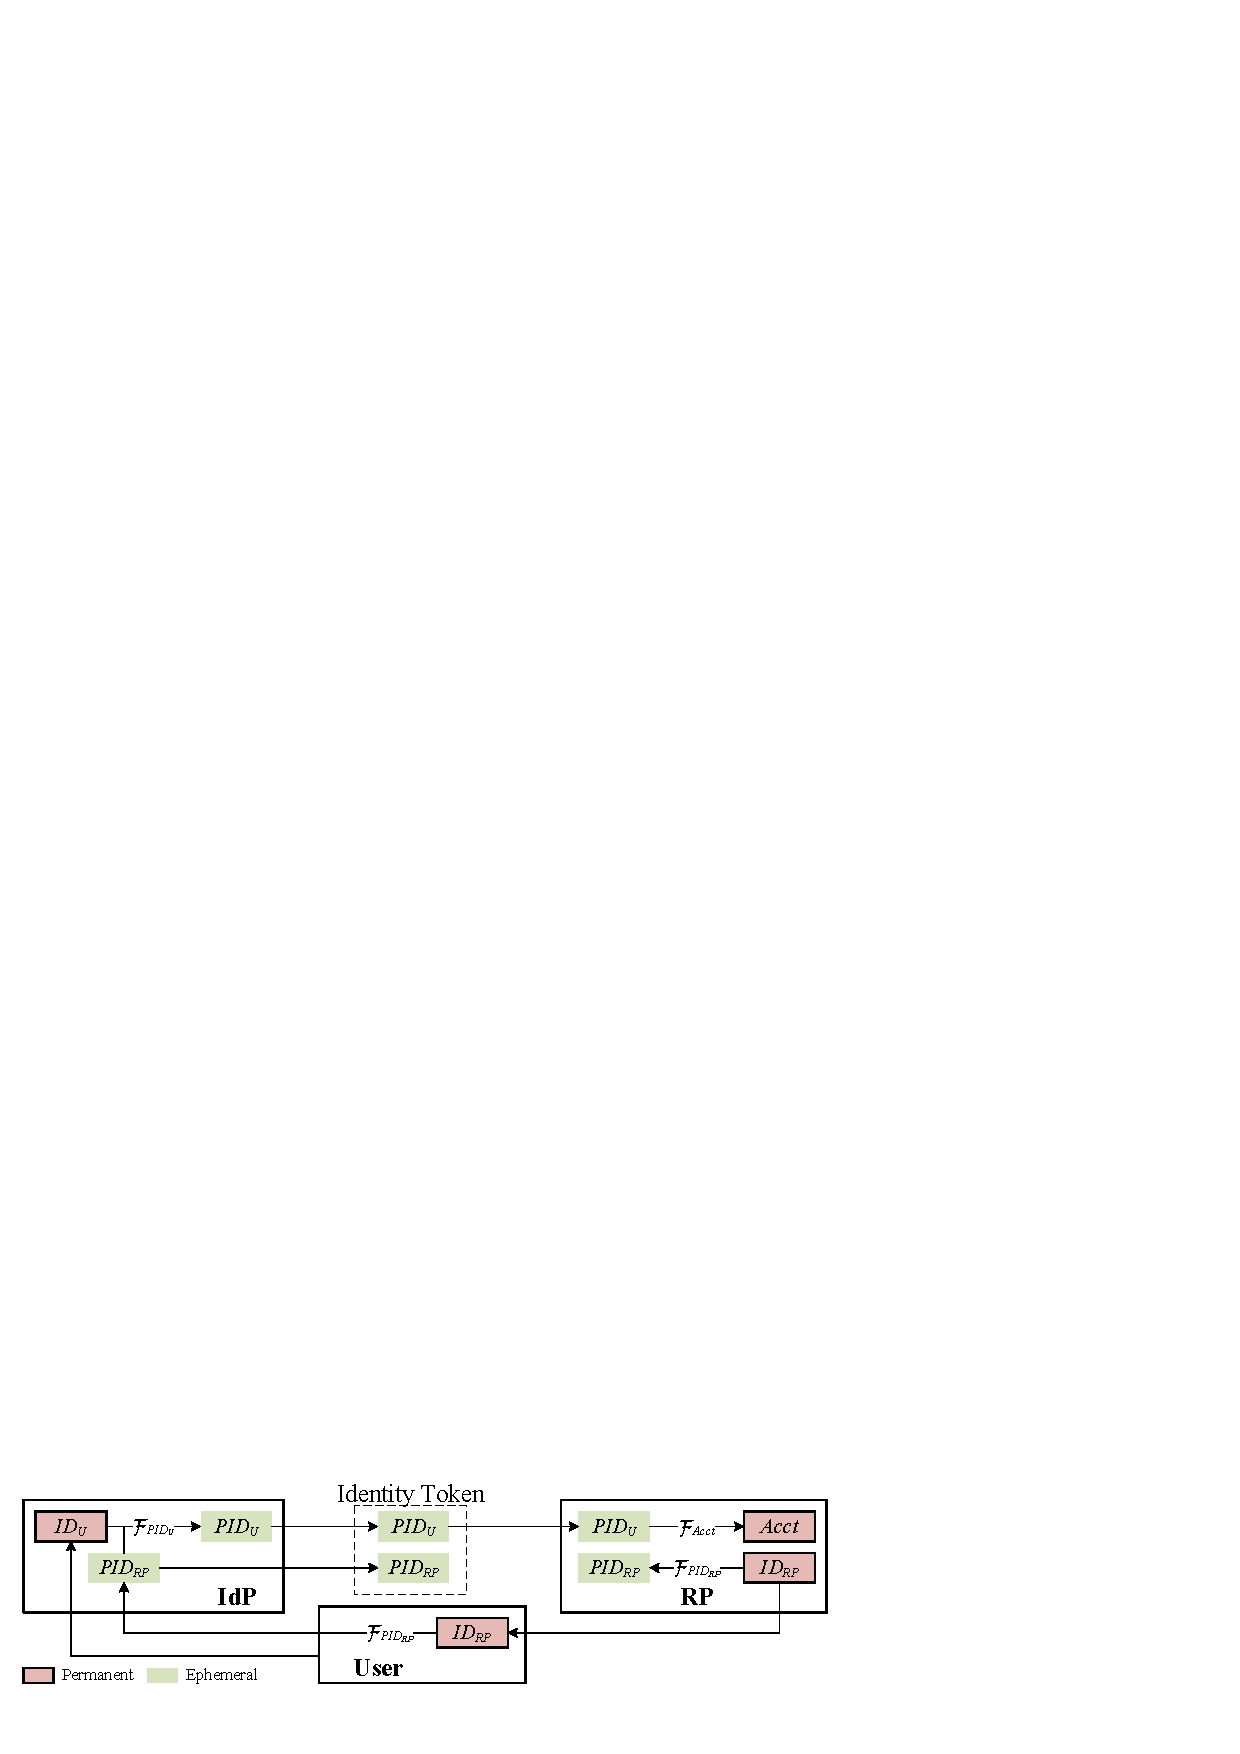
\includegraphics[width=1.00\linewidth]{fig/IDCorrelation.pdf}
  \caption{Identity transformations in \usso} %privacy-preserving SSO}
  \label{fig:IDCorrelation}
\end{figure}

For RP designation, $PID_{RP}$ should be associated \emph{uniquely} with the target RP.
For user identification, with \emph{ephemeral} $PID_{U}^l$ in each login, the designated RP should be able to derive a locally-unique \emph{permanent} account  (i.e., $Acct$) for the user at this RP.
In order to prevent IdP-based login tracing, it is essential to ensure that the IdP does not obtain any information about $ID_{RP}$ from any $PID_{RP}^l$.
Thus, in a user's multiple logins visiting an RP,
\emph{independent} $PID_{RP}^l$s
and \emph{independent} $PID_U^l$s should be generated:
The IdP should not be able to link multiple logins visiting a given RP, while the RP's identity is kept unknown to the IdP. If $PID_U^l$ is not completely independent of each other, it is possible for the IdP to link multiple logins visiting a certain RP.
Finally, to prevent RP-based identity linkage,
the RP should not obtain any information about $ID_U$ from any $PID_{U,j}$, which implies that $PID_{U,j}$ for visiting different RPs should also be independent of each other.

We propose the following identity transformations in a login initiated by a user to visit an RP in privacy-preserving SSO:
\vspace{-\topsep}
\begin{itemize}
\setlength{\topsep}{0pt}
\setlength{\partopsep}{0pt}
\setlength{\itemsep}{0pt}
\setlength{\parsep}{0pt}
\setlength{\parskip}{0pt}
\item
$\mathcal{F}_{Acct\ast}(ID_{U}, ID_{RP}) = Acct$, determining a user' account at an RP.
% by the IdP which assigns $ID_{U}$ and $ID_{RP}$.
Given $ID_U$ and $ID_{RP}$, $Acct$ is %\emph{permanent} and
\emph{unique} at this RP.

\item
$\mathcal{F}_{PID_{RP}}(ID_{RP}) = PID_{RP}$, calculated by the user.
In the IdP's view,
$\mathcal{F}_{PID_{RP}}()$ is a one-way function and $PID_{RP}$
is \emph{indistinguishable} from random variables.
\item
$\mathcal{F}_{PID_U}(ID_U, PID_{RP}) = PID_{U}$, calculated by the IdP.
In the target RP's view,
    $\mathcal{F}_{PID_U}()$ is a one-way function and $PID_{U}$ is \emph{indistinguishable} from random variables.
\item
$\mathcal{F}_{Acct}(PID_{U}, PID_{RP}) = Acct$, calculated by the target RP.
That is, in the user's multiple logins visiting the RP,
    $Acct = \mathcal{F}_{Acct\ast}(ID_{U}, ID_{RP})$ is always derived.
\end{itemize}



